\documentclass[class=article, crop=false]{standalone}
\usepackage[subpreambles=false]{standalone}
\usepackage{import}
% Options for packages loaded elsewhere
\PassOptionsToPackage{unicode}{hyperref}
\PassOptionsToPackage{hyphens}{url}


\usepackage{amsmath,amssymb}
\usepackage{lmodern}
\usepackage{iftex}
\ifPDFTeX
  \usepackage[T1]{fontenc}
  \usepackage[utf8]{inputenc}
  \usepackage{textcomp} % provide euro and other symbols
\else % if luatex or xetex
  \usepackage{unicode-math}
  \defaultfontfeatures{Scale=MatchLowercase}
  \defaultfontfeatures[\rmfamily]{Ligatures=TeX,Scale=1}
\fi
% Use upquote if available, for straight quotes in verbatim environments
\IfFileExists{upquote.sty}{\usepackage{upquote}}{}
\IfFileExists{microtype.sty}{% use microtype if available
  \usepackage[]{microtype}
  \UseMicrotypeSet[protrusion]{basicmath} % disable protrusion for tt fonts
}{}
\makeatletter
\@ifundefined{KOMAClassName}{% if non-KOMA class
  \IfFileExists{parskip.sty}{%
    \usepackage{parskip}
  }{% else
    \setlength{\parindent}{0pt}
    \setlength{\parskip}{6pt plus 2pt minus 1pt}}
}{% if KOMA class
  \KOMAoptions{parskip=half}}
\makeatother
\usepackage{xcolor}
\usepackage[margin=1in]{geometry}
\usepackage{color}
\usepackage{fancyvrb}
\newcommand{\VerbBar}{|}
\newcommand{\VERB}{\Verb[commandchars=\\\{\}]}
\DefineVerbatimEnvironment{Highlighting}{Verbatim}{commandchars=\\\{\}}
% Add ',fontsize=\small' for more characters per line
\usepackage{framed}
\definecolor{shadecolor}{RGB}{248,248,248}
\newenvironment{Shaded}{\begin{snugshade}}{\end{snugshade}}
\newcommand{\AlertTok}[1]{\textcolor[rgb]{0.94,0.16,0.16}{#1}}
\newcommand{\AnnotationTok}[1]{\textcolor[rgb]{0.56,0.35,0.01}{\textbf{\textit{#1}}}}
\newcommand{\AttributeTok}[1]{\textcolor[rgb]{0.77,0.63,0.00}{#1}}
\newcommand{\BaseNTok}[1]{\textcolor[rgb]{0.00,0.00,0.81}{#1}}
\newcommand{\BuiltInTok}[1]{#1}
\newcommand{\CharTok}[1]{\textcolor[rgb]{0.31,0.60,0.02}{#1}}
\newcommand{\CommentTok}[1]{\textcolor[rgb]{0.56,0.35,0.01}{\textit{#1}}}
\newcommand{\CommentVarTok}[1]{\textcolor[rgb]{0.56,0.35,0.01}{\textbf{\textit{#1}}}}
\newcommand{\ConstantTok}[1]{\textcolor[rgb]{0.00,0.00,0.00}{#1}}
\newcommand{\ControlFlowTok}[1]{\textcolor[rgb]{0.13,0.29,0.53}{\textbf{#1}}}
\newcommand{\DataTypeTok}[1]{\textcolor[rgb]{0.13,0.29,0.53}{#1}}
\newcommand{\DecValTok}[1]{\textcolor[rgb]{0.00,0.00,0.81}{#1}}
\newcommand{\DocumentationTok}[1]{\textcolor[rgb]{0.56,0.35,0.01}{\textbf{\textit{#1}}}}
\newcommand{\ErrorTok}[1]{\textcolor[rgb]{0.64,0.00,0.00}{\textbf{#1}}}
\newcommand{\ExtensionTok}[1]{#1}
\newcommand{\FloatTok}[1]{\textcolor[rgb]{0.00,0.00,0.81}{#1}}
\newcommand{\FunctionTok}[1]{\textcolor[rgb]{0.00,0.00,0.00}{#1}}
\newcommand{\ImportTok}[1]{#1}
\newcommand{\InformationTok}[1]{\textcolor[rgb]{0.56,0.35,0.01}{\textbf{\textit{#1}}}}
\newcommand{\KeywordTok}[1]{\textcolor[rgb]{0.13,0.29,0.53}{\textbf{#1}}}
\newcommand{\NormalTok}[1]{#1}
\newcommand{\OperatorTok}[1]{\textcolor[rgb]{0.81,0.36,0.00}{\textbf{#1}}}
\newcommand{\OtherTok}[1]{\textcolor[rgb]{0.56,0.35,0.01}{#1}}
\newcommand{\PreprocessorTok}[1]{\textcolor[rgb]{0.56,0.35,0.01}{\textit{#1}}}
\newcommand{\RegionMarkerTok}[1]{#1}
\newcommand{\SpecialCharTok}[1]{\textcolor[rgb]{0.00,0.00,0.00}{#1}}
\newcommand{\SpecialStringTok}[1]{\textcolor[rgb]{0.31,0.60,0.02}{#1}}
\newcommand{\StringTok}[1]{\textcolor[rgb]{0.31,0.60,0.02}{#1}}
\newcommand{\VariableTok}[1]{\textcolor[rgb]{0.00,0.00,0.00}{#1}}
\newcommand{\VerbatimStringTok}[1]{\textcolor[rgb]{0.31,0.60,0.02}{#1}}
\newcommand{\WarningTok}[1]{\textcolor[rgb]{0.56,0.35,0.01}{\textbf{\textit{#1}}}}
\usepackage{graphicx}
\makeatletter
\def\maxwidth{\ifdim\Gin@nat@width>\linewidth\linewidth\else\Gin@nat@width\fi}
\def\maxheight{\ifdim\Gin@nat@height>\textheight\textheight\else\Gin@nat@height\fi}
\makeatother
% Scale images if necessary, so that they will not overflow the page
% margins by default, and it is still possible to overwrite the defaults
% using explicit options in \includegraphics[width, height, ...]{}
\setkeys{Gin}{width=\maxwidth,height=\maxheight,keepaspectratio}
% Set default figure placement to htbp
\makeatletter
\def\fps@figure{htbp}
\makeatother
\setlength{\emergencystretch}{3em} % prevent overfull lines
\providecommand{\tightlist}{%
  \setlength{\itemsep}{0pt}\setlength{\parskip}{0pt}}
\setcounter{secnumdepth}{-\maxdimen} % remove section numbering
\ifLuaTeX
\usepackage[bidi=basic]{babel}
\else
\usepackage[bidi=default]{babel}
\fi
\babelprovide[main,import]{ngerman}
% get rid of language-specific shorthands (see #6817):
\let\LanguageShortHands\languageshorthands
\def\languageshorthands#1{}
\ifLuaTeX
  \usepackage{selnolig}  % disable illegal ligatures
\fi
\IfFileExists{bookmark.sty}{\usepackage{bookmark}}{\usepackage{hyperref}}
\IfFileExists{xurl.sty}{\usepackage{xurl}}{} % add URL line breaks if available
\urlstyle{same} % disable monospaced font for URLs
\hypersetup{
  pdftitle={Brownsche Molekularbewegung},
  pdfauthor={Milena Mensching, Justus Weyers},
  pdflang={de},
  hidelinks,
  pdfcreator={LaTeX via pandoc}}

\title{Brownsche Molekularbewegung}
\author{Milena Mensching, Justus Weyers}
\date{2023-01-04}

\begin{document}


\hypertarget{simulation}{%
\section{Simulation}\label{simulation}}

Mittels einer Simulation soll versucht werden, die durch die Diffusion
bedingte Bewegung von Polystyrolpartikeln unter verschiedenen
Bedingungen nachzustellen. In der Simulation lassen sich die Anzahl von
Stößen und die Partikelanzahl einstellen. Auch die Simulationsdauer kann
verändert werden, diese haben wir aber konstant bei einer Länge von fünf
Sekunden belassen. Für die drei eingestellten Kombinationen ergaben sich
folgende Histogramme für die Schrittweite eines ``Random-walks'':

\begin{figure}
\centering
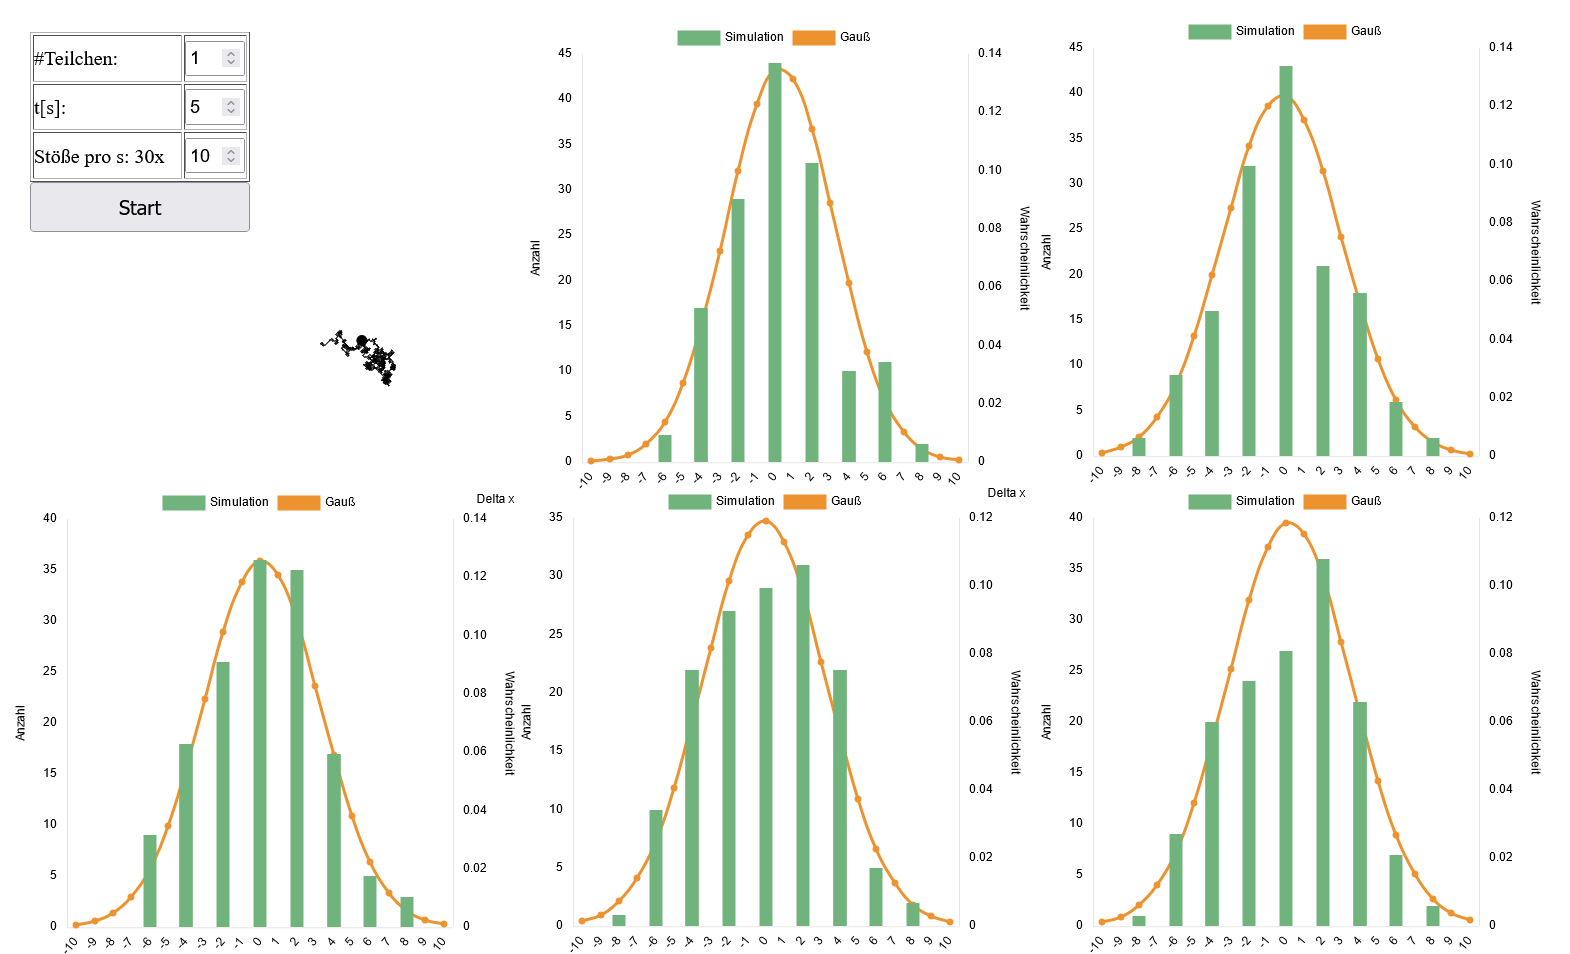
\includegraphics[width=\textwidth,height=0.25\textheight]{Daten/a.png}
\caption{Simulation 1. 1 Teilchen, 5 Sekunden, 300 Stöße pro s}
\end{figure}

\begin{figure}
\centering
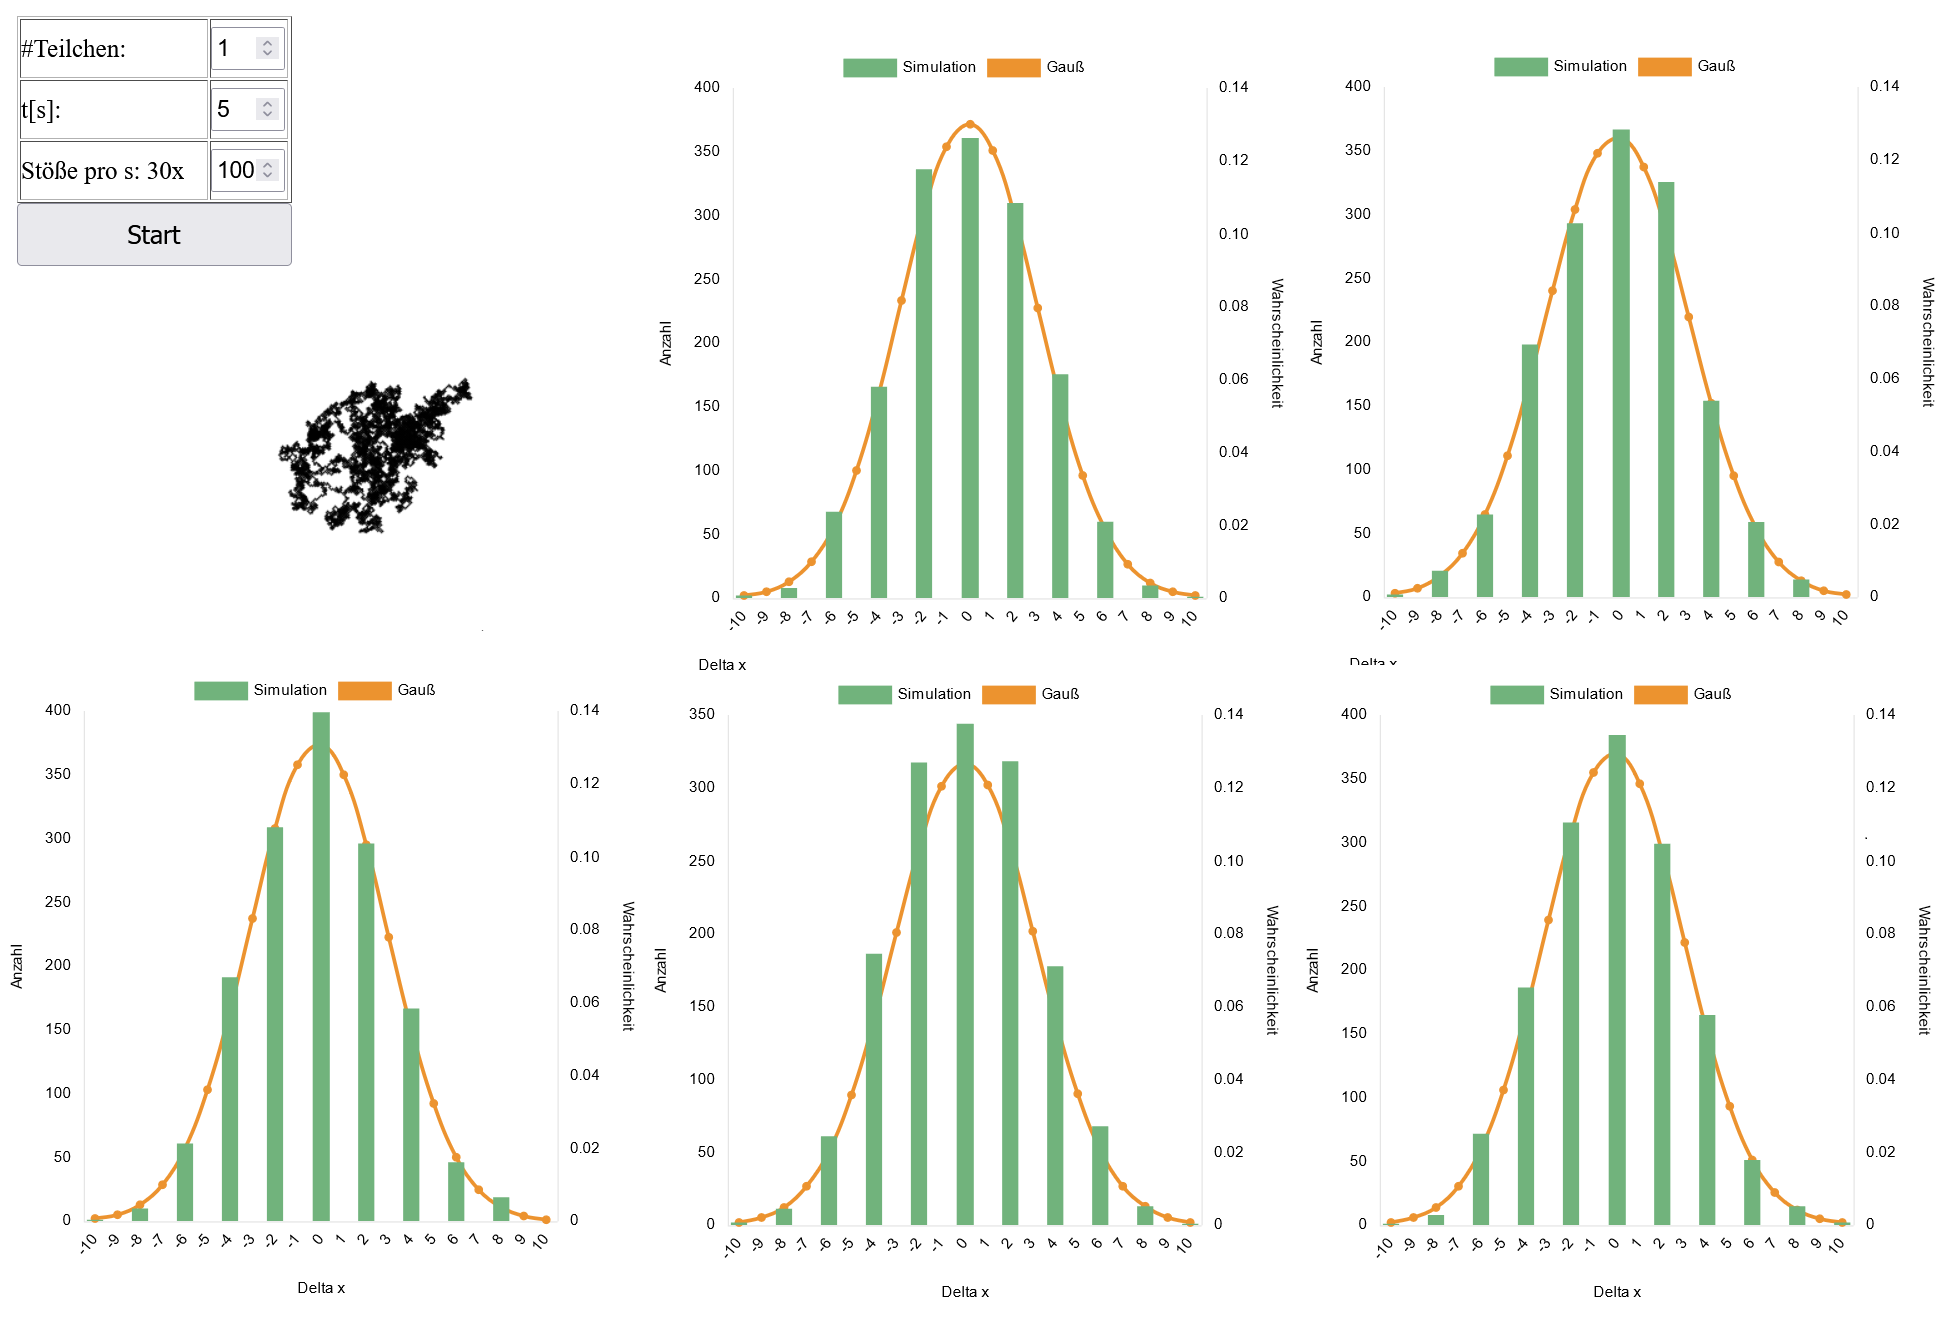
\includegraphics[width=\textwidth,height=0.25\textheight]{Daten/b2.png}
\caption{Simulation 2. 1 Teilchen, 5 Sekunden, 3000 Stöße pro s}
\end{figure}

\begin{figure}
\centering
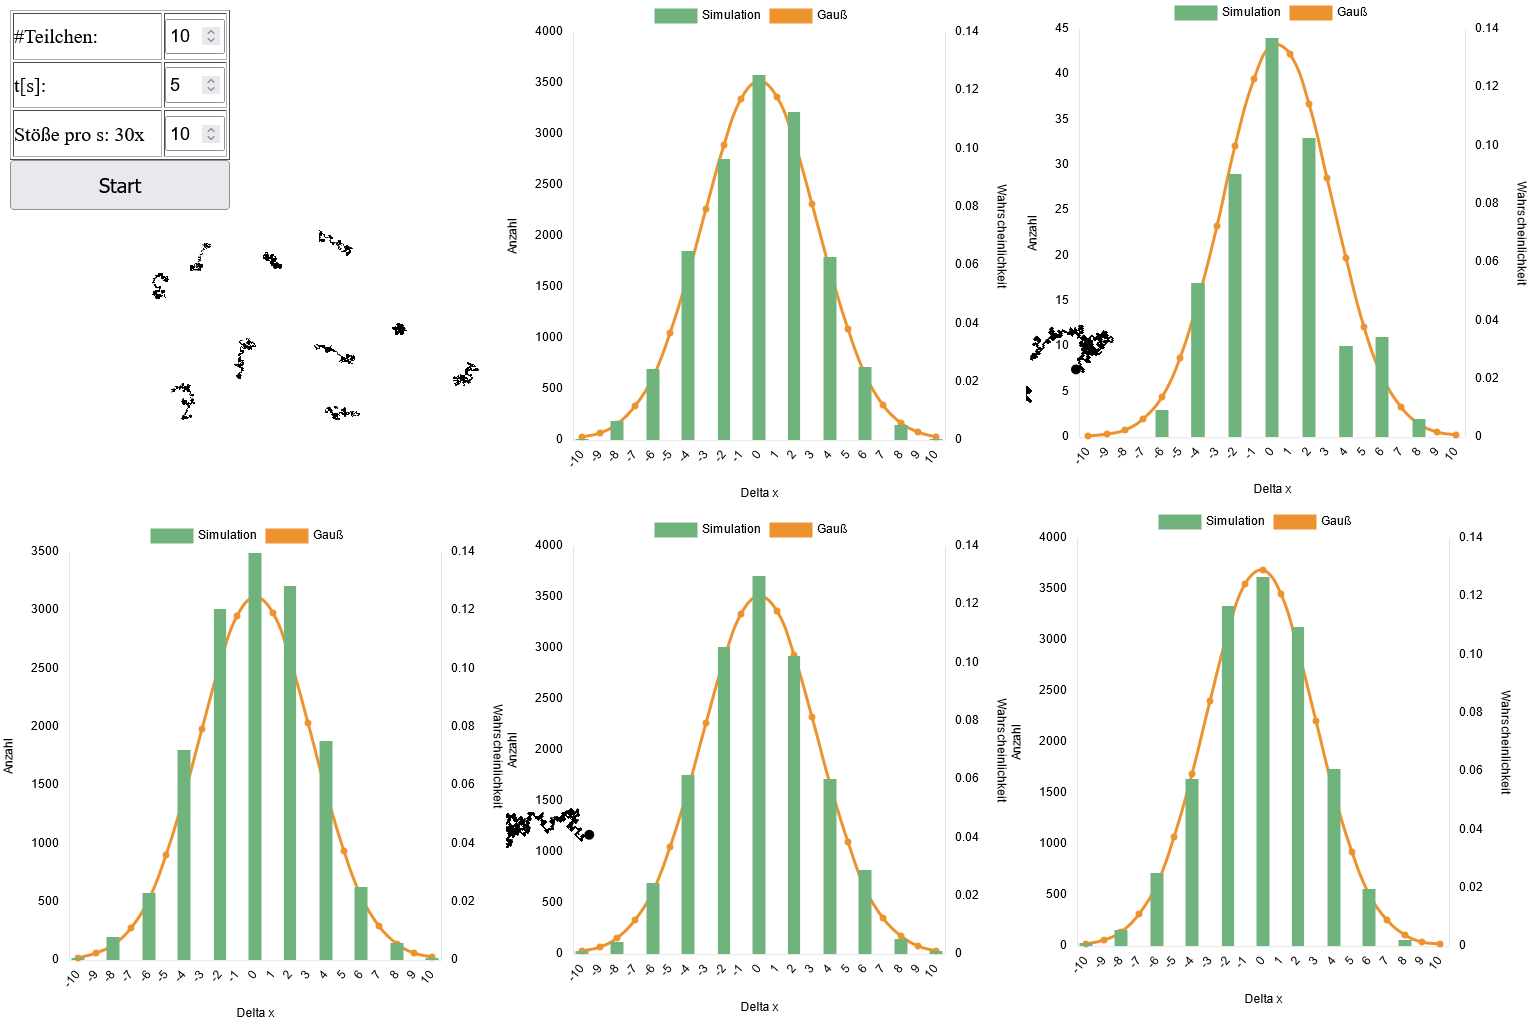
\includegraphics[width=\textwidth,height=0.25\textheight]{Daten/c.png}
\caption{Simulation 3. 10 Teilchen, 5 Sekunden, 300 Stöße pro s}
\end{figure}

Für die Auswertung der Simulationsergebnisse werden verallgemeinernd und
vereinfachend die optischen Gesamteindrücke der Histogramme verglichen.
Wird das gemacht, fällt auf, dass die Histogramme für die Versuche b)
und c) am meisten normalverteilt aussehen. Die Verteilungen entsprechen
im Allgemeinen ganz gut den eingezeichneten Normalverteilungen (in
Orange) für den ermittelten Mittelwert und die Standardabweichung der
Daten. Der Mittelwert und die Standardabweichung wurden in der
Simulation nicht ausgegeben, aber es ist erkennbar, dass der Mittelwert
bei allen Histogrammen bei Null liegt und die Standardabweichung ein
gutes Maß angenommen hat.

Die Ergebnisse von Versuch a) fallen gegenüber den Ergebnissen aus b)
und c) in puncto Normalverteiltheit etwas ab. Grund für dieses etwas
schlechter ausfallende Ergebniss in a) ist vermutlich, dass hier mit den
jeweiligen Minimalwerten der Versuchsreihe (1 Teilchen bei nur 10x30
Stößen pro Sekunde) gerechnet wurde. In b) und c) fällt immer jeweils
einer dieser beiden Werte wesentlich höher aus (jeweils um einen Faktor
10).

Dass zwischen b) und c) kaum Unterschiede im Ergebnis, dafür aber in den
Simulationsparametern bestehen, könnte durch das Ergodentheorem
erklärbar sein, wonach es für das Ergebnis einer Random-walk-Betrachtung
auf dasselbe hinausläuft, ob eine große Anzahl von Teilchen mit wenigen
Stößen pro Sekunde, oder eine kleine Menge von Teilchen mit vielen
Stößen pro Sekunde beobachtet wird.

\hypertarget{experiment}{%
\section{Experiment}\label{experiment}}

\hypertarget{thema}{%
\subsection{Thema}\label{thema}}

Bestimmung dere Diffusionskonstanten eines Polystyrolpartikels, sowie
die Berechnung der Boltzmann- und Avogadrokonstanten.

\hypertarget{material}{%
\subsection{Material}\label{material}}

\begin{itemize}
\item{Mikropartikel (Polystyrol) Suspension in Wasser}
\item{Lichtmikroskop mit Objektträger}
\item{Deckplättchen}
\item{Thermometer}
\item{Zur Messung und Auswertung wurden folgende Computerprogramme benutzt: ThorCam, Tracker, SciDAVis, Python, R.}
\end{itemize}

\hypertarget{versuchsaufbau-und-durchfuxfchrung}{%
\subsection{Versuchsaufbau und
Durchführung}\label{versuchsaufbau-und-durchfuxfchrung}}

\begin{figure}
\centering
\includegraphics[width=\textwidth,height=0.2\textheight]{Bilder/Objektträger.png}
\caption{Mikroskop mit Probe}
\end{figure}

Auf einen Objektträger wurde ein Tropfen einer Mikropartikel
(Polystyrol) Suspension in Wasser gegeben. Zwei Deckplättchen wurden
neben den Tropfen, und eines mittig auf die anderen beiden positioniert
und unter das Mikroskop gelegt. Die Polystyrolpartikel (PSP) wurden
scharf gestellt. Als Vergrößerung wurde 40/0.65 gewählt.

\hypertarget{durchfuxfchrung}{%
\subsection{Durchführung}\label{durchfuxfchrung}}

Mit Hilfe einer Mikroskopkamera und des Programms ``ThorCam'' wird die
Projektion auf dem Bildschirm sichtbar. Eine Zeitreihe über den Zeitraum
von hundert Sekunden und im Umfang von 100 Bildern wurde von den PSP
automatisch, mittels ``ThorCam'', erstellt. Über die Messunsicherheit
der Länge der Zeitintervalle ist nichts bekannt.

Nach Aufnehmen der Messreihe wurde die Temperatur im Lichtgang des
Mikroskopes für ca. 20 Sekunden gemessen. Diese betrug ca. 21,7°C. Die
Messunsicherheit liegt bei
\(u_{Temp}=\frac{0,1^{\circ}C}{2\sqrt{6}}= 0,020^{\circ}C\). Danach
wurde mit Hilfe des Programms ``Tracker'' die Position des Teilchens
ausgewertet. Dafür wird in einem Datensatz von 100 Bildern das
``Teilchen of interest'' mit dem Cursor markiert.

Neben dieser Methode wurde eine zweite Auswertung des Bildmaterials
vorgenommen. Diese bestand darin, mittels eines Pythonscripts die
Mittelpunkte aller 17 PSP in allen 100 Einzelbildern zu bestimmen. Das
Ergebnis dieses Verfahrens war eine große Datei mit den Koordinaten
aller 17 PSP-Mittelpunkte in allen 100 Bildern. Es wurde darauf
verzichtet, diese hier abzudrucken, stattdessen werden die Ergebnisse in
Abbildung 5 grafisch dargestellt. Mit diesen Daten wird
weitergearbeitet.

\hypertarget{fehlerbetrachtung}{%
\subsection{Fehlerbetrachtung}\label{fehlerbetrachtung}}

Eine Unsicherheit der Methodik besteht in der Umrechnung der Bildpunkte
in Meter. Eine zweite Unsicherheit besteht in der Auflösung des Bildes.
Durch die verwendete Methode konnte eine manuelle Verfolgung der PSP
umgangen werden. Diese computervisuelle Methodik sollte zu kleineren
Fehlern führen.

\hypertarget{beobachtungen}{%
\subsection{Beobachtungen}\label{beobachtungen}}

Zu Beginn werden die zurückglegten Wege aller PSP im Bildausschnitt
geplottet. Ein einzelner, ausgewählter Partikel (NR. 2) wird
exemplarisch genauer dargestellt, indem dessen Bewegungspfad einzeln in
einem höheren Maßstab geplottet wird.

\begin{figure}
\centering
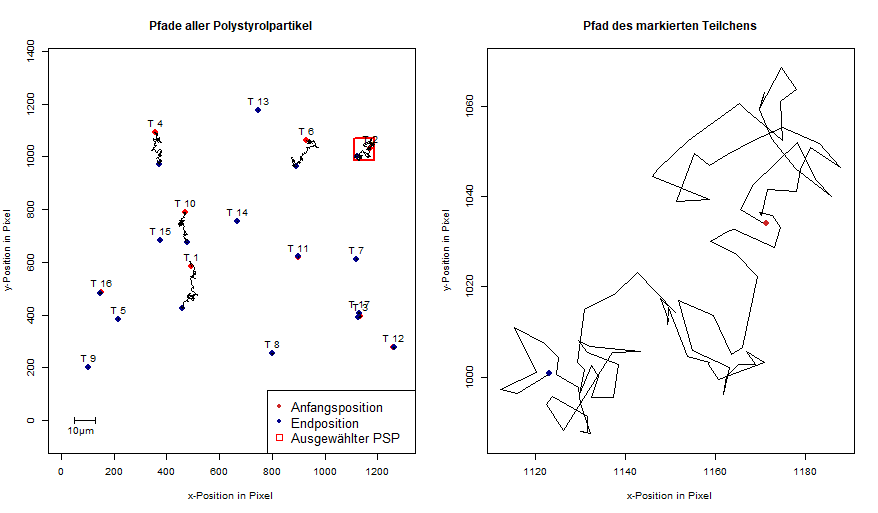
\includegraphics[width=\textwidth,height=0.4\textheight]{code/Plots/Raum.png}
\caption{Auf diesen zwei Plots sind die Positionen aller bzw. eines
markierten PSP im zeitlichen Verlauf zu sehen. Die Aufnahmedauer betrug
100 s mit 1 fps. Die PSP wurden zudem nummeriert.}
\end{figure}

Auf Abbildung 5 ist erkennbar, dass die 17 beobachteten PSP sich in
ihren zurückgelegten Wegen deutlich unterscheiden. Während 12 PSP sich
praktisch nicht von ihrer Ausgangsposition bewegt haben, ist bei sechs
Teilchen eine deutliche Abweichung zwischen Anfangs- und Endposition
auszumachen. Es ist nicht verwunderlich, dass viele Partikel keinen
räumlichen Versatz aufweisen. Netto sollte die Bewegung aller
Randomwalks zusammengenommen zu einem Verharren jedes Teilchens an
seinem Ursprung führen, Abweichungen durch die Standardabweichungen sind
möglich. Es ist aber auch möglich, dass diese Teilchen an den
Glaspättchen kleben. Zwar sind auch für die scheinbar unbewegten
Teilchen Bewegungen bestimmt worden, diese sind aber mikroskopisch kaum
nachweisbar und könnten ein Resultat der Unsicherheit beim verwendeten
computervisuellen Auswertungsverfahren sein.

Interpretationsspielraum geben die zurückgelegten Pfade der fünf anderen
Teilchen (T 1, 2, 4, 6, 10, siehe Abbildung 5). Jene ``viel bewegten
Teilchen'' weisen trotz aller Zufälligkeit der einzelnen Random-walks
eine gewisse Tendenz zu einer Bewegung entgegen der y-Achse auf. Hier
stellt sich die Frage, ob neben der diffusiven Bewegungskomponente auch
eine advektive Transportkomponente einen Einfluss auf die
Teilchenbewegung hatte. Dies wäre eine weitere mögliche Fehlerquelle.

\hypertarget{umrechnung-der-messwerte-in-meter}{%
\subsubsection{Umrechnung der Messwerte in
Meter}\label{umrechnung-der-messwerte-in-meter}}

Im nächsten Schritt können die ermittelten Werte für die Diffusionspfade
von Pixel in Meter umgerechnet werden. Hierbei ist der Maßstab der
aufgenommenen Bilder vonnöten. Dafür werden die PSP selbst verwendet,
von denen bekannt ist, dass deren Durchmesser \(2 \mu m\) beträgt. Beim
Zählen der Bildpixel ist darauf geachtet worden, die Originalauflösung
zu verwenden, in der auch die Berechnung der Schrittweiten berechnet
wurde.

\begin{figure}
\centering
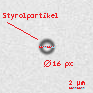
\includegraphics[width=\textwidth,height=0.28\textheight]{Bilder/styrolpartikel.png}
\caption{Polystyrolpartikel mit dem Durchmesser 2µm. Der Durchmesser ist
in Pixel abgemessen und beträgt 16 Pixel.}
\end{figure}

Aus dem Zusammenhang, dass sechzehn Bildpixel zwei Mikrometern
entsprechen, folgt für die Kantenlänge eines Pixels eine Länge von
\(0,125 \mu m\). Die kleinste ablesbare Skala in dem Bild ist der
Durchmesser von \(2\mu m\) des PSP. Für die Unsicherheit der Kantenlänge
eines Pixels folgt so
\(u_{Pixellänge} = \frac{1}{16}\cdot \frac{2\mu m}{2\sqrt{6}} = 0,026\mu m\).

\begin{Shaded}
\begin{Highlighting}[]
\CommentTok{\# Berechnung der Kantenlänge eines Pixels}
\DecValTok{2}\SpecialCharTok{*}\DecValTok{10}\SpecialCharTok{**}\NormalTok{(}\SpecialCharTok{{-}}\DecValTok{6}\NormalTok{)}\SpecialCharTok{/}\DecValTok{16}
\end{Highlighting}
\end{Shaded}

\begin{verbatim}
## [1] 1.25e-07
\end{verbatim}

\begin{Shaded}
\begin{Highlighting}[]
\CommentTok{\# Berechnung Unsicherheit der Kantenlänge:}
\DecValTok{2}\SpecialCharTok{*}\DecValTok{10}\SpecialCharTok{**}\NormalTok{(}\SpecialCharTok{{-}}\DecValTok{6}\NormalTok{)}\SpecialCharTok{/}\NormalTok{(}\DecValTok{16}\SpecialCharTok{*}\DecValTok{2}\SpecialCharTok{*}\FunctionTok{sqrt}\NormalTok{(}\DecValTok{6}\NormalTok{))}
\end{Highlighting}
\end{Shaded}

\begin{verbatim}
## [1] 2.551552e-08
\end{verbatim}

\hypertarget{statistische-untersuchung}{%
\subsubsection{Statistische
Untersuchung}\label{statistische-untersuchung}}

Nach dieser Umrechnung kann mit statistischen Mitteln versucht werden,
weitere Aussagen über das Diffusionsverhalten der PSP zu treffen. Im
weiteren Verlauf sollen dann die Diffusionskonstante, die
Boltzmannkonstante und die Avogadrokonstante anhand eines ausgewählten
Teilchens berechnet werden.

Zunächst wird also die Random-walk-Schrittweite (RWS) des ausgesuchten
Teilchens 2 berechnet. Die Berechnung findet nur in einer räumlichen
Dimension, der x-Dimension, statt. Die RWS wird berechnet, indem die
x-Postition des Bildes \(i\) von der x-Position des Bildes \(i+1\)
abgezogen wird. Die Berechnung findet in R statt:

\begin{Shaded}
\begin{Highlighting}[]
\CommentTok{\# Einlesen der x{-}Positionen aller Teilchen aus dem erhobenen Datensatz}
\NormalTok{x\_meter }\OtherTok{\textless{}{-}} \FunctionTok{read.csv}\NormalTok{(}\StringTok{\textquotesingle{}code/Tabellen/x\_meter.csv\textquotesingle{}}\NormalTok{)}

\DocumentationTok{\#\#\# Funktion zur Berechnung der RWS}
\NormalTok{calculateDistance1D }\OtherTok{=} \ControlFlowTok{function}\NormalTok{(vector)\{}
\NormalTok{  shift\_vector }\OtherTok{=} \FunctionTok{c}\NormalTok{(}\DecValTok{0}\NormalTok{, vector[}\DecValTok{1}\SpecialCharTok{:}\NormalTok{(}\FunctionTok{length}\NormalTok{(vector)}\SpecialCharTok{{-}}\DecValTok{1}\NormalTok{)])}
\NormalTok{  dist }\OtherTok{=}\NormalTok{ vector}\SpecialCharTok{{-}}\NormalTok{shift\_vector}
\NormalTok{  dist[}\DecValTok{1}\NormalTok{] }\OtherTok{=} \DecValTok{0}
  \FunctionTok{return}\NormalTok{(dist)}
\NormalTok{\}}

\CommentTok{\# Berechnung der RWS von Teilchen 2}
\NormalTok{RWS }\OtherTok{\textless{}{-}} \FunctionTok{calculateDistance1D}\NormalTok{(x\_meter}\SpecialCharTok{$}\NormalTok{X}\FloatTok{.2}\NormalTok{)}
\end{Highlighting}
\end{Shaded}

Die RWS in x-Richtung von Teilchen 2 kann grafisch veranschaulicht
werden. Dies erfolgt mittels eines Histogramms, in dem die Häufigkeiten
bestimmter RWS aufgetragen ist.

\begin{figure}
\centering
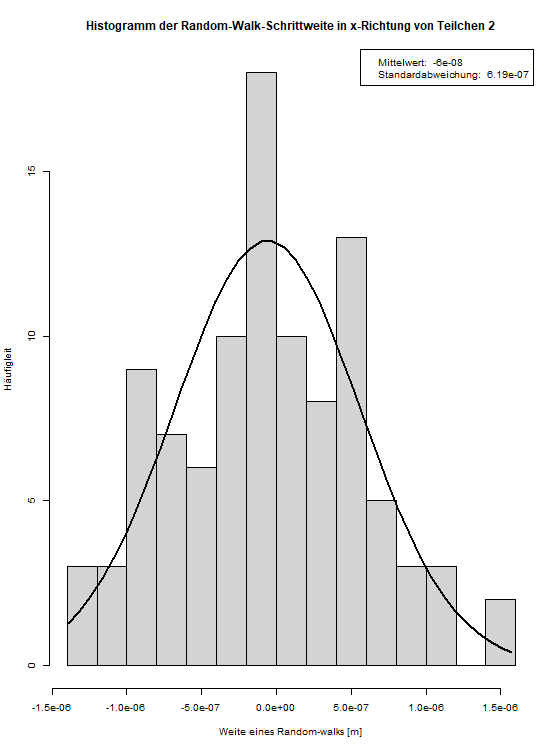
\includegraphics[width=\textwidth,height=0.5\textheight]{code/Plots/Teilchen2.png}
\caption{Das Histogramm zeigt die Häufigkeit der Schrittweiten pro
Random-walk für Teilchen 2}
\end{figure}

Das Histogramme sieht normalverteilt aus.

\begin{Shaded}
\begin{Highlighting}[]
\FunctionTok{shapiro.test}\NormalTok{(RWS)}
\end{Highlighting}
\end{Shaded}

\begin{verbatim}
## 
##  Shapiro-Wilk normality test
## 
## data:  RWS
## W = 0.99134, p-value = 0.7713
\end{verbatim}

Ein Shapiro-Wilk Test unter der Nullhypohese der Normalverteiltheit
liefert einen p-Wert von \(p = 0,7713\). Die Mittelwerte der Bewegung
beträgt \(-6\cdot10^{-8}m\). Dass dieser von Null abweicht, liegt
entweder daran, dass das Teilchen nicht über einen genügend langen
Zeitraum beobachtet wurde, oder aber auch daran, dass neben der
Diffusion auch andere Bewegungskomponenten (Advektion) auf den PSP
wirkte. In Abbildung 4 ist ebenfalls ersichtlich, das Teilchen 2
insgesamt eine leichte Tendenz zu Bewegungen entgegen der x-Achse hatte.

\hypertarget{auswertung}{%
\subsection{Auswertung}\label{auswertung}}

\hypertarget{berechnung-der-diffusionskonstante}{%
\subsubsection{Berechnung der
Diffusionskonstante}\label{berechnung-der-diffusionskonstante}}

Mittels der folgender Formel kann für Teilchen 2 die Diffusionskonstante
\(D\) berechnet werden: \[D=\frac{\sigma^2}{2t}\] Mit:

\begin{itemize}
\item $\sigma$: Standardabweichung der Schrittweite eines Random-walks für ein PSP
\item $t$: Zeitintervall zwischen zwei Bildaufnahmen ($t=1s=const.$).
\end{itemize}

Nun kann die Standardabweichung aus den Werten der RWS-Serie berechnet
werden.

\begin{Shaded}
\begin{Highlighting}[]
\CommentTok{\# Standardabweichung x{-}Verschiebung von Teilchen 2}
\NormalTok{sigma }\OtherTok{=} \FunctionTok{sd}\NormalTok{(RWS) }\CommentTok{\#m}
\NormalTok{sigma}
\end{Highlighting}
\end{Shaded}

\begin{verbatim}
## [1] 6.18505e-07
\end{verbatim}

Der Fehler der Standardabweichung berechnet sich als Quotient aus
Standardabweichung und der Anzahl von Messwerten (\(n=100\)).

\begin{Shaded}
\begin{Highlighting}[]
\CommentTok{\# Fehler der Standardabweichung}
\NormalTok{u\_sigma }\OtherTok{=} \FunctionTok{sd}\NormalTok{(RWS)}\SpecialCharTok{/}\DecValTok{100} \CommentTok{\#m}
\NormalTok{u\_sigma}
\end{Highlighting}
\end{Shaded}

\begin{verbatim}
## [1] 6.18505e-09
\end{verbatim}

Unter der Annahme, dass die Bewegung hinreichend lange beobachtet wurde
beträgt die mittlere Verschiebung \(\sigma\), bzw. Schrittweite
\(\delta\) bzw. Standardabweichung der Verschiebung \(\Delta x\):
\(\sigma = (6.185 \pm 0.062 )\cdot 10^{-7}m = (0.6185 \pm 0.0062 )\mu m\).

Nun kann die Diffusionskonstante berechnet werden (in
\(\frac{m^2}{s}\)):

\begin{Shaded}
\begin{Highlighting}[]
\CommentTok{\# Berechnung der Diffusionskonstanten für Teilchen 2}
\NormalTok{D }\OtherTok{=} \FunctionTok{sd}\NormalTok{(RWS)}\SpecialCharTok{\^{}}\DecValTok{2}\SpecialCharTok{/}\NormalTok{(}\DecValTok{2}\SpecialCharTok{*}\DecValTok{1}\NormalTok{) }\CommentTok{\#m\^{}2/s}
\NormalTok{D}
\end{Highlighting}
\end{Shaded}

\begin{verbatim}
## [1] 1.912742e-13
\end{verbatim}

Auch die Unsicherheit der Diffusionskonstante kann berechnet werden. Da
über die Unsicherheit der vom Computer bestimmten Zeitintervalle nichts
weiter bekannt ist wird \(u_t\) als null angenommen.
\[u_D = \sqrt{(\frac{\partial D}{\partial \sigma}\cdot u_{\sigma})^2 + \frac{\partial D}{\partial t}\cdot u_{t})^2}= \sqrt{(\frac{2\sigma}{2t}\cdot u_{\sigma})^2+(\frac{\sigma^2}{2t^2}\cdot u_t)^2}\]

\begin{Shaded}
\begin{Highlighting}[]
\CommentTok{\# Berechnung der Unsicherheit der Diffusionskonstanten für Teilchen 2}
\NormalTok{u\_D }\OtherTok{=} \FunctionTok{sqrt}\NormalTok{( (}\DecValTok{2}\SpecialCharTok{*}\NormalTok{sigma}\SpecialCharTok{/}\DecValTok{2}\SpecialCharTok{*}\NormalTok{u\_sigma)}\SpecialCharTok{**}\DecValTok{2} \SpecialCharTok{+}\NormalTok{ (sigma}\SpecialCharTok{**}\DecValTok{2}\SpecialCharTok{/}\DecValTok{2}\SpecialCharTok{*}\DecValTok{1}\SpecialCharTok{**}\DecValTok{2}\SpecialCharTok{*}\DecValTok{0}\NormalTok{)}\SpecialCharTok{**}\DecValTok{2}\NormalTok{ ) }\CommentTok{\#m\^{}2/s}
\NormalTok{u\_D}
\end{Highlighting}
\end{Shaded}

\begin{verbatim}
## [1] 3.825484e-15
\end{verbatim}

Damit wurde für Partikel 2 eine Diffusionskonstante von
\(D=(191.2 \pm 3.8)\cdot 10^{-15} \frac{m^2}{s}\) bestimmt.

\hypertarget{berechnung-der-boltzmannkonstante}{%
\subsubsection{Berechnung der
Boltzmannkonstante}\label{berechnung-der-boltzmannkonstante}}

Die Boltzmannkonstante soll über die Einstein-Smoluchowski-Gleichung
berechnet werden:
\[DC = k_B\cdot T \Leftrightarrow k_B = \frac{DC}{T} \Leftrightarrow k_B = \frac{D\cdot 6\pi \eta r}{T}\]
Mit:

\begin{itemize}
  \item $k_B$: Boltzmannkonstante
  \item $D$: Diffusionskonstante $(0.6185 \pm 0.0062 )\frac{\mu m^2}{s}$
  \item $C$: Stokessche Reibungskonstante ($C=6\pi \eta r$)
  \item $T$: Temperatur $(21,700 \pm 0,020)^{\circ}C$
  \item $\eta$: danamische Viskosität von Wasser bei $20^{\circ}C$: $1002\cdot 10^{-6} \frac{kg}{ms}$
  \item $r$: Radius des PSP $2\mu m$
\end{itemize}

Die Berechnung der ermittelten Boltzmannkonstante ergibt, mit der
Einheitenbetrachtung
\([\frac{\frac{m^2}{s}*\frac{kg}{ms}*m}{K} = \frac{kg\cdot m^2}{K\cdot s^2}= \frac{J}{K}]\):

\begin{Shaded}
\begin{Highlighting}[]
\NormalTok{eta }\OtherTok{=} \FloatTok{1002e{-}6} \CommentTok{\# m\^{}2/s}
\NormalTok{r }\OtherTok{=} \FloatTok{1e{-}6} \CommentTok{\# m }
\NormalTok{Temp }\OtherTok{=} \FloatTok{21.7} \SpecialCharTok{+} \FloatTok{273.15}
\NormalTok{kB }\OtherTok{=}\NormalTok{ (D}\SpecialCharTok{*}\DecValTok{6}\SpecialCharTok{*}\NormalTok{pi}\SpecialCharTok{*}\NormalTok{eta}\SpecialCharTok{*}\NormalTok{r)}\SpecialCharTok{/}\NormalTok{(Temp) }\CommentTok{\#kg*m\^{}2/(s\^{}2*K)}
\NormalTok{kB}
\end{Highlighting}
\end{Shaded}

\begin{verbatim}
## [1] 1.225248e-23
\end{verbatim}

Die Unsicherheit der ermittelten Boltzmannkonstante \(u_{kB}\) errechnet
sich als:
\[u_{kB} = \sqrt{(\frac{\partial k_B}{\partial D}\cdot u_D)^2 + (\frac{\partial k_B}{\partial T}\cdot u_T)^2}\]
\[\sqrt{(\frac{6\pi \eta r}{T}\cdot u_D)^2+(\frac{D\cdot 6\pi \eta r}{T^2} \cdot u_T)^2}\]

\begin{Shaded}
\begin{Highlighting}[]
\NormalTok{u\_T }\OtherTok{=} \FloatTok{0.020} \CommentTok{\# K}
\FunctionTok{sqrt}\NormalTok{(((}\DecValTok{6}\SpecialCharTok{*}\NormalTok{pi}\SpecialCharTok{*}\NormalTok{eta}\SpecialCharTok{*}\NormalTok{r)}\SpecialCharTok{/}\NormalTok{(Temp)}\SpecialCharTok{*}\NormalTok{u\_D)}\SpecialCharTok{**}\DecValTok{2}\SpecialCharTok{+}\NormalTok{((D}\SpecialCharTok{*}\DecValTok{6}\SpecialCharTok{*}\NormalTok{pi}\SpecialCharTok{*}\NormalTok{eta}\SpecialCharTok{*}\NormalTok{r)}\SpecialCharTok{/}\NormalTok{(Temp}\SpecialCharTok{**}\DecValTok{2}\NormalTok{)}\SpecialCharTok{*}\NormalTok{u\_T)}\SpecialCharTok{\^{}}\DecValTok{2}\NormalTok{)}
\end{Highlighting}
\end{Shaded}

\begin{verbatim}
## [1] 2.450511e-25
\end{verbatim}

In diesem Versuch wurde also eine Boltzmannkonstante von
\(k_B = (1,225 \pm 0,025) \cdot 10^{-23} \frac{J}{K}\) bestimmt.

\hypertarget{berechnung-der-avogadrokonstante}{%
\subsubsection{Berechnung der
Avogadrokonstante}\label{berechnung-der-avogadrokonstante}}

Es gilt das allgemeine Gesetz:

\begin{equation*}
R=N_A*k_B \leftrightarrow N_A = \frac{R}{k_B}
\end{equation*} \noindent \(R\) = universelle Gaskonstante =
\(8,314 \frac{J}{mol\cdot K}\)\\
\noindent \(N_A\) = Avogadrokonstante\\
\noindent \(k_B\) = Boltzmannkonstante

Damit ergibt sich mit der zuvor ermittelten Boltzmannkonstante von
\(k_B = (1,225 \pm 0,025) \cdot 10^{-23} \frac{J}{K}\) ein Bestwert von:

\begin{equation*}
N_A = \frac{R}{k_B} = \frac{8,314 \frac{J}{mol\cdot K}}{1,225 \cdot 10^{-23} \frac{J}{K}} \approx 6.786939\cdot 10^{23} \frac{1}{mol}
\end{equation*}

Die Unsicherheit ergibt sich mit:

\begin{equation*}
u_{NA}= \frac {\partial N_A}{\partial k_B} \cdot u_{kB} 
= \vert - \frac{R}{k_B^2} \cdot u_{kB}\vert 
= \frac{8,314 \frac{J}{mol\cdot K}}{(1,225 \cdot 10^{-23} \frac{J}{K})^2} \cdot 0,025 \cdot 10^{-23} \frac{J}{K} \approx 0,14 \cdot 10^{23} \frac{1}{mol}
\end{equation*}

\begin{Shaded}
\begin{Highlighting}[]
\FloatTok{8.314}\SpecialCharTok{/}\NormalTok{(}\FloatTok{1.225}\SpecialCharTok{*}\DecValTok{10}\SpecialCharTok{**{-}}\DecValTok{23}\NormalTok{) }\CommentTok{\#Bestwert Avogadrokonstante}
\end{Highlighting}
\end{Shaded}

\begin{verbatim}
## [1] 6.786939e+23
\end{verbatim}

\begin{Shaded}
\begin{Highlighting}[]
\FloatTok{8.314}\SpecialCharTok{/}\NormalTok{((}\FloatTok{1.225}\SpecialCharTok{*}\DecValTok{10}\SpecialCharTok{**{-}}\DecValTok{23}\NormalTok{)}\SpecialCharTok{**}\DecValTok{2}\NormalTok{)}\SpecialCharTok{*}\FloatTok{0.025}\SpecialCharTok{*}\DecValTok{10}\SpecialCharTok{**{-}}\DecValTok{23} \CommentTok{\#Unsicherheit}
\end{Highlighting}
\end{Shaded}

\begin{verbatim}
## [1] 1.38509e+22
\end{verbatim}

Die Avogadrokonstante ergibt sich folglich mit
\(N_A = (6.79 \pm 0.14) \cdot 10^{23} \frac{1}{mol}\).

\hypertarget{interpretation}{%
\subsection{Interpretation}\label{interpretation}}

Obwohl sowohl der Literaturwert für die Boltzmannkonstante
(\(k_B = 1,380 \cdot 10^{-23} \frac{J}{K}\)), als auch der Literaturwert
der Avogadrokonstante (\(N_A = 6,022 \cdot 10^{23} \frac{1}{mol}\))
nicht in die von uns bestimmten Intervalle fallen, liegen beide
ermittelten Werte in der richtigen Größenordnung und nahe am
Literaturwert. Sie können daher als ganz gute Näherungen betrachtet
werden.

\end{document}
